\begin{tikzpicture}[overlay, remember picture]
    \node[anchor=north west, rotate=0, gray, font=\tiny, text width=\paperwidth] at (current page.south west)  [xshift=0, yshift=0.75cm] {
    [1] L. Amico et al., Entanglement in Many-Body Systems, Reviews of Modern Physics 80, no. 2 (2008)
    };
\end{tikzpicture}


\begin{figure}[h]
    \centering
    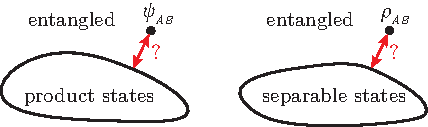
\includegraphics{imgs/Asset 2.pdf}
    %\caption{}
    %\label{fig:}
\end{figure}

\phantom{42}


% \onslide<1>{
\textbf{Multipartite} entanglement: <<dinstance>> from product states \vspace{-2mm}
\begin{equation*}
    E_g(\Psi) \overset{\mathrm{def}}{=} - \log_2 \max_{\Phi \in \mathcal{S}} |\bk{\Psi}{\Phi}|^2,
\end{equation*}
% \phantom{42}
% with = $S(\rho || \rho') = \tr \rho (\ln \rho - \ln \rho')$.
% }


\onslide<2>{
Or average purity  \vspace{-5mm}
\begin{equation*}
    \sub{E}{gl} \overset{\mathrm{def}}{=}  2 - \frac{2}{N} \sum_{j=1}^N \tr \rho_j^2
\end{equation*}
% *reduces to $S(\rho)$ in the case of pure bi-partite states.
}